\section{Problematika zobrazovania GPS trás}

\indent \indent Zobrazovanie \acrshort{gps} trás je zásadné pre množstvo aplikácií, od navigácie a mapovania až po analýzu údajov o pohybe. \acrshort{gps} zariadenia získavajú informácie z družíc a používajú trianguláciu na určenie polohy. Tieto informácie sa zhromažďujú vo forme súradníc spolu s časovými údajmi\cite{Hegarty2017}. 

Trasu získame spojením súradníc získaných z \acrshort{gps} zariadenia. Problém nastáva, keď sú \acrshort{gps} signály ovplyvnené faktormi ako sú terén, počasie alebo rôznymi prekážkami. Ovplyvnené signály môžu viesť k nepresným alebo chybným údajom\cite{Hegarty2017}. Spojením chybných údajov získame nepresnú trasu, ktorá leží mimo skutočnej, po ktorej sme sa reálne pohybovali.

Keď sa rovnakou trasou prechádza opakovane, údaje z GPS zariadenia môžu vykazovať variabilitu. Pri vizualizácii trás, ktoré sú zaznamenané prejdením rovnakej trasy, môže dôjsť k prekrývaniu a neprehľadnosti v dôsledku odchýlok a nepresností. Prekrývajúce sa trasy je možné vidieť na obrázku \ref{fig:neprehladne-trasy}. Z dôvodu nepresnosti je zložité rozpoznať detaily mapy, ako aj cestnú sieť, čo sťažuje identifikáciu jednotlivých trás.

\begin{figure}[H]
    \centering
    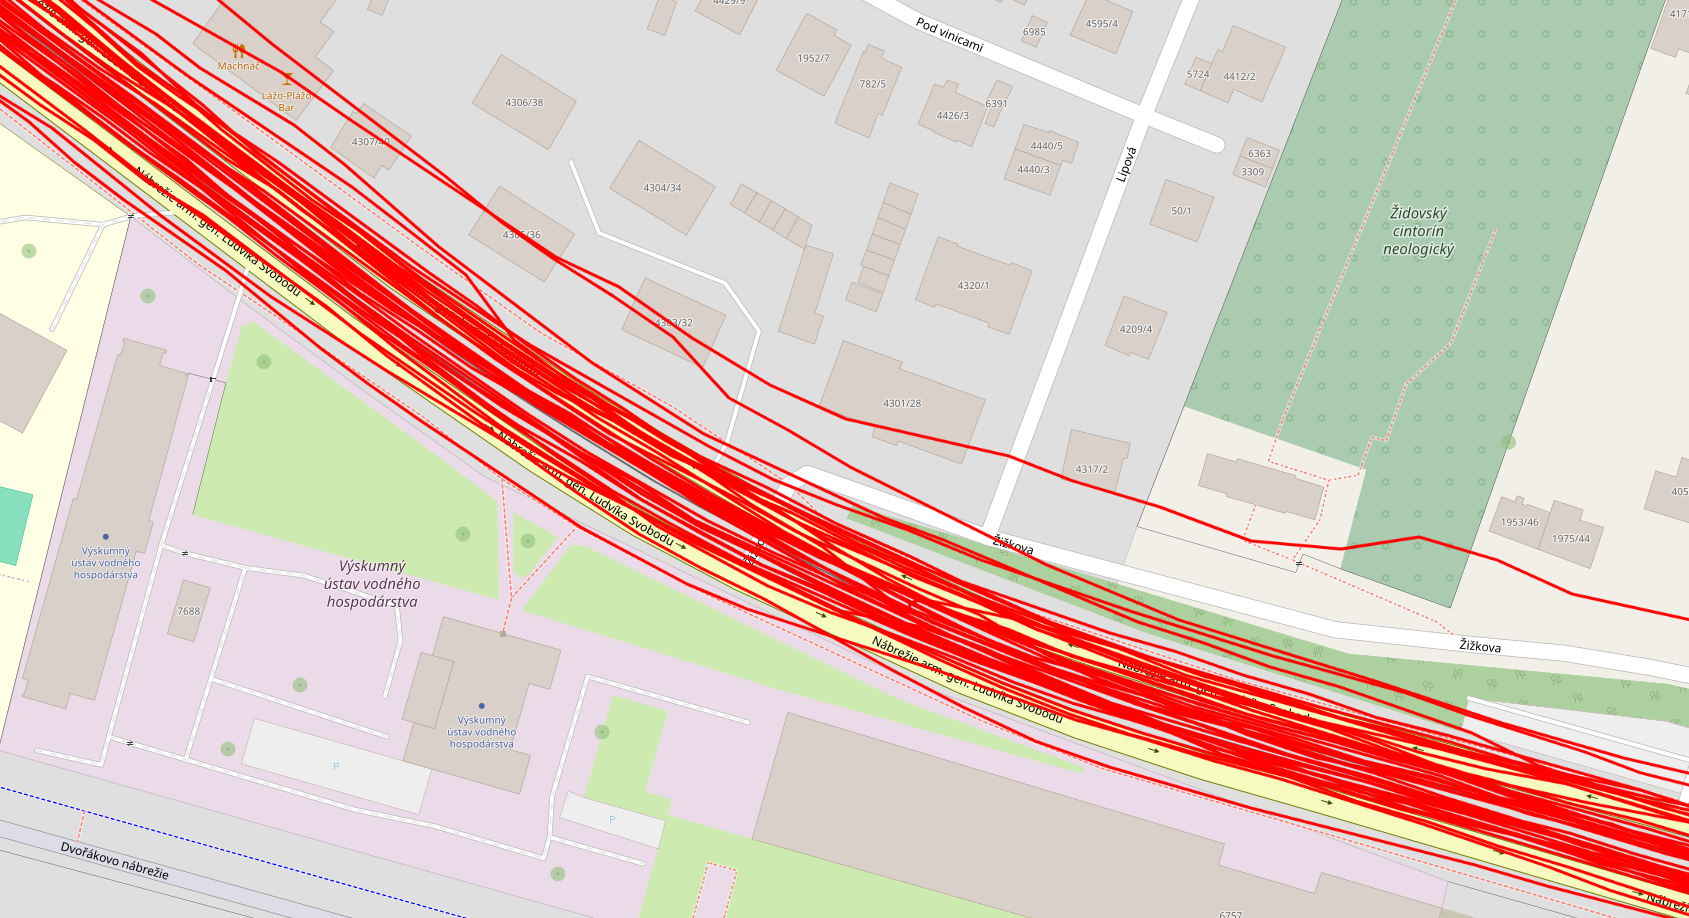
\includegraphics[width=.8 \textwidth]{img/problematika_gps/neprehladne_trasy.png}
    \caption{Neprehľadne zobrazené trasy.}
    \label{fig:neprehladne-trasy}
  \end{figure}

  Pre zlepšenie viditeľnosti a sprehľadnenie mapy použijeme metódu pripnutia trás k cestnej sieti, nazývanú \textit{map-match}. Vďaka tejto metóde budú všetky trasy ležať na cestnej sieti. Všetky trasy, ktoré sme získali pri pohybe po rovnakej trase budú prekryté. Po prejdení myšou po trase sa zobrazí okno, ktoré bude obsahovať názvy trás.